\documentclass[a4paper, 10pt]{report}

\usepackage{url}
\usepackage{algorithm}
\usepackage[noend]{algpseudocode}
\usepackage[english]{babel}
\usepackage[utf8x]{inputenc}

\usepackage{graphicx}
\usepackage[a4paper]{geometry}
\usepackage{palatino}

%\usepackage{fontspec}
%\setromanfont{Times New Roman}
%\setsansfont{Lucida Sans}
%\setmonofont{Consolas}
\usepackage{listings}
\lstset{
	language=Java,
	basicstyle=\footnotesize\ttfamily,
	frame=single,
	tabsize=2,
	numbers=left
}  
\usepackage[T1]{fontenc}
\usepackage[scaled]{beramono}
\usepackage{amsmath}
\usepackage[toc,page]{appendix}
\usepackage{enumitem}
\setlist[enumerate]{itemsep=0mm}

\begin{document}

\begin{titlepage}

\newcommand{\HRule}{\rule{\linewidth}{0.5mm}} 
\center
 
\textsc{\LARGE Imperial College London}\\[1.5cm] % Name of your university/college
\textsc{\Large Department of Computing}\\[0.5cm] % Major heading such as course name
\textsc{\large Summer Research Project}\\[0.5cm] % Minor heading such as course title

\HRule \\[0.4cm]
{ \LARGE 
  \textbf{Multi-Pumping on Maxeler Platform} \\[0.2cm]
  \large A General Study on Multi-Pumping\\ Implementation, Application and Compiler }\\[0.3cm] % Title of your document
\HRule \\[1.5cm]
 
\begin{minipage}[t]{0.4\textwidth}
\begin{flushleft}
\textbf{Author:}\\
Vincent \textsc{Zhao}\\ % Your name
\emph{Peking University}
\end{flushleft}
\vfill
\end{minipage}
~
\begin{minipage}[t]{0.4\textwidth}
\begin{flushright}
\textbf{Supervisor:} \\
Dr. Timothy \textsc{Todman} \\% Supervisor's Name
\emph{Imperial College London} \\[0.2cm]
Prof. Wayne \textsc{Luk}\\
\emph{Imperial College London}
\end{flushright}
\vfill
\end{minipage}\\[2cm]

{\large \today}\\[2cm]

\vfill % Fill the rest of the page with whitespace
\end{titlepage}

\begin{abstract}
This research report contains both general and detailed explanation about the research project for this summer. It will start from multi-pumping, a technique which could save design resource usage without affecting the speed. And illustrate several designs which are based on, or be optimized by multi-pumping. SpMV is the most important one, it has much more aspects than those pure multi-pumping work, and it will be described in detail. At last, there's an approach to do multi-pumping by using Ruby, an HDL language which is quite simple and precise. I have finished several revision on Ruby compiler, and the work which makes the compiler to have the ability to translate Ruby into multiple kernel MaxJ code is interesting both in software algorithm and hardware design.
\end{abstract}
\newpage

\tableofcontents

\chapter{Multi-Pumping}

About multi-pumping, the details have been described in \cite{Canis:2013}. My work is mainly focusing on how to utilize multi-pumping technique on Maxeler platform, with MaxJ HLS language. 

% Here I should describe what is the multi-pumping problem, from it's origin
\section{Background} 
Multi-pumping is a technique which could reduce the resource usage of a design, and in most cases, with nearly no speed affected. Multi-pumping is a problem originated from resouce sharing problem, which is mainly focusing on how to use only part of the previous resource usage without affecting the performance. And the way to solve this problem is highly dependent on scheduling, we need to schedule which operations should cooperate on one single resource. But it should be quite hard to get good resource sharing result from pure scheduling method as it's an NP-hard problem, and there're many heuristic method to optimize the algorithm's time complexity. 

The basic idea of multi-pumping is to run 2 or more operations on one circuit component, with faster clock rate. For example, if we want to do 2 multiplications in one clock cycle, without multi-pumping, we need to use 2 multipliers for one cycle. But now we could run one multiplier at 2x clock rate, and obviously, this multiplier could handle 2 multiplications. Despite of this, we 
need one more component: multiplexer, to steer different inputs to the multiplier in different clock cycle. In the following figure, the 2x rate clock signal will be transferred to the multiplexer, and in different clock cycle, the input will be steered differenly. 

\begin{figure}[h!]
  \caption{A multi-pumped square circuit.}
  \centering
    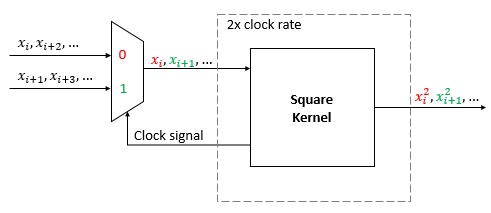
\includegraphics[width=0.7\textwidth]{square-mp}
\end{figure}


So multi-pumping could be regarded as an optimization to scheduling problem, from this point of view, we could implicitly schedule 2 or more operations to one resource unit, with double, triple or more clock cycles. And this is the approach from \cite{Canis:2013}, they revised their own LegUp, an open source HLS system, by changing its scheduling algorithm. Their scheduling algorithm will take care of MPM(multi-pumped multiplier)'s usage.

But what if there's no way to change the underneath multi-pumping algorithm? And what if we want to do multi-pumping on much complexer components rather than simple multiplier? Like a read port of RAM, or a group of DSPs. These are my focusing points of my multi-pumping project, with Maxeler platform, I've devised a template to do multi-pumping \textit{explicitly} on code-level, without changing the HLS algorithm. Several experiments could support the correctness of this approach.
 
\section{Brief introduction to MaxJ}
MaxJ is a programming language which supports Maxeler HLS system. It's based on Java. It's initial idea is to build hardware by running these MaxJ java code and generate a hardware configuration file. Each MaxJ project could be devided into 2 parts, MaxJ's \textbf{Kernel} will generate the hardware, and the \textbf{Manager} will handle the connections and configurations among kernels and host CPUs. Here's a simple MaxJ code snippet:

\begin{lstlisting}[caption=Non multi-pumped kernel example,float]
public NoMPKernel extends Kernel {
	NoMPKernel(KernelParameters params) {
		super(params);
		
		DFEVar x0 = io.input("x0", dfeUInt(32));
		DFEVar y0 = io.input("y0", dfeUInt(32));
		DFEVar x1 = io.input("x1", dfeUInt(32));
		DFEVar y1 = io.input("y1", dfeUInt(32));
		
		io.output("o1", x0 * y0, dfeUInt(32));
		io.output("o1", x0 * y0, dfeUInt(32));
	}
}
\end{lstlisting}

This kernel will simply multiply 4 inputs: $x_0$ and $y_0$, $x_1$ and $y_1$. And outputs them to different output streams. Each tick this kernel will take 1 element from each stream. And the manager will handle input and output connected to this kernel. It's obvious that this kernel needs 2 multipliers, as there're 2 \textit{asterisks} on line 10 and line 11.

\begin{figure}[h!]
  \caption{DFE architecture}
  \centering
    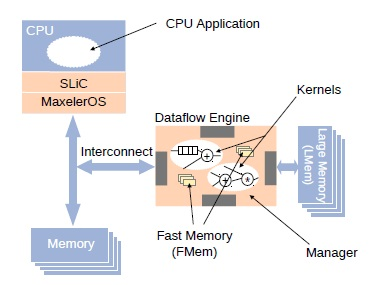
\includegraphics[width=0.7\textwidth]{dfe-arch}
\end{figure}

More precisely, the generated output of MaxJ is called DataFlow Engine(DFE, see Figure 1.2), which take inputs and outputs as streams, and process them in a dataflow pattern. Kernels that generated could be regared as processing units in the dataflow, and manager handles how the dataflow connected to each other. MaxJ generate a configuration file of Maxeler DFE which is called Maxfile, which could be used to generate interface between host CPU and DFE, and set up bitstreams on FPGA hardware.

In the next sections, we'll focus on 1 problem: how could we transform a non multi-pumped kernel code in MaxJ, to a multi-pumped one? It seems not so hard at first glance, but there do have some tricky details we need to take care of. And by using the methodology I've devised and illustrated later, we could build multi-pumping project in the code level systematically

\section{Multi-pumping MaxJ methodology}
There're 3 steps to transforma non multi-pumped kernel to a multi-pumped one:
\begin{enumerate}
\item \textbf{Split kernel by clock rate}: we put components with different clock rate into different kernels.
\item \textbf{Steer inputs and outputs}: In kernels with faster clock rate, we need to steer input data in different clock cycles.
\item \textbf{Configure manager}: Including clock frequency configuration and kernel connection details.
\end{enumerate}

\subsection{Split kernel by clock rate}
In order to write Multi-pumping code explicitly, you need to assign different clock rate for different components. And according to MaxJ's convention and restriction, one kernel could only have one clock rate, which could be set in manager. If you have an original MaxJ design which only contains one kernel, the first thing you need to do to multi-pump it is splitting it into multiple kernels, and different kernel has different clock rate.

We could describe our multi-pumping design in a DFE style(Figure 1.3). There're several 1x clock rate kernel handles slow operations, and take or push input to 2x clock rate kernel. This 2x clock rate kernel could have contained many DSPs, or some BRAMs with read or write ports, or some other fast components.

\begin{figure}[h!]
  \caption{DFE Multi-Pumping}
  \centering
    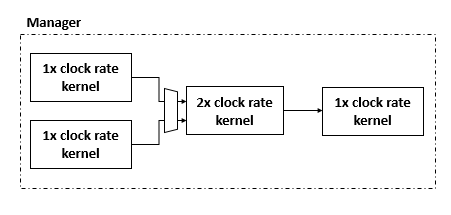
\includegraphics[width=0.8\textwidth]{dfe-mp-wireframe}
\end{figure}

\subsection{Steer inputs and outputs}
We could do this in the manager level, by using \texttt{mux} method of manager class. However, it's more intuitive to do it in kernel, by using simple counter. We could revise our original Non multi-pumped code like this:

\begin{lstlisting}[caption=Non multi-pumped kernel example, float]
DFEVar counter = control.count.simpleCounter(2);

DFEVar x0 = io.input("x0", dfeUInt(32), counter === 0);
DFEVar y0 = io.input("y0", dfeUInt(32), counter === 0);
DFEVar x1 = io.input("x1", dfeUInt(32), counter === 1);
DFEVar y1 = io.input("y1", dfeUInt(32), counter === 1);

io.output("o1", x0 * y0, dfeUInt(32), counter === 0);
io.output("o1", x0 * y0, dfeUInt(32), counter === 1);
....
\end{lstlisting}

Here \texttt{===} could be regarded as "take value and compare with". For the counter, it will count from 0 to 1 and loop back to 0. So it's equivilant to use a multiplexer which take clock signal as input. And the output will also be controlled by this counter value.

\subsection{Configure manager}
The most important thing to configure in manager is the clock rate. Under MaxJ's context, all the clock rate will be set only for stream, and the kernel clock rate could be derived from its in/out stream clock setting. For example, if the input stream of one kernel is 100MHz, then this kernel will run as 100MHz. It follows the dataflow nature of Maxeler DFE platform.

And also, currently there's no way to specify ratio timing constraints, such as one stream is 2 times faster than the other stream, so we need to set clock value explicitly: global stream is 100MHz and the multi-pumped kernels' stream will be 100n MHz.

\section{Experimental Study}
Their are 2 main studies of multi-pumped MaxJ code: One is called \textit{inner square product}, which will do $x_i^2 \times y_i^2$ for 2 input streams, the other one is called \textit{window summation}, which calculates summation of a window of array, and the array's value will be gathered from ROM. The latter one could be written in:

$$Sum = \sum_{i=0}^W rom[index[i]] $$

Where $W$ is the window width, and $index$ is the input stream which contains address of $rom$ to read. The code of these 2 project could be referenced from this repository \footnote{Github repository folder: \url{https://goo.gl/uxJ9xO}}, and the experimental data has also be included there.

For the first design, it's focusing on integrating kernel with many DSPs to one multi-pumped kernel. And for the second one, it shows a noval implementation of multi-pumping on ROM read, which could save a lot of memory space on board as one copy of BRAM could only support 2 read ports at the same time. With multi-pumping, we could do 4, 8 and more(although this may not be a good idea) read ports in one tick. In this figure, the multi-pumped version(C=2) has nearly half of the BRAM resource usage than non multi-pumped one(C=1), and the frequecies are nearly the same.

\begin{figure}[h!]
  \caption{ROM Read Port Multi-Pumping}
  \centering
    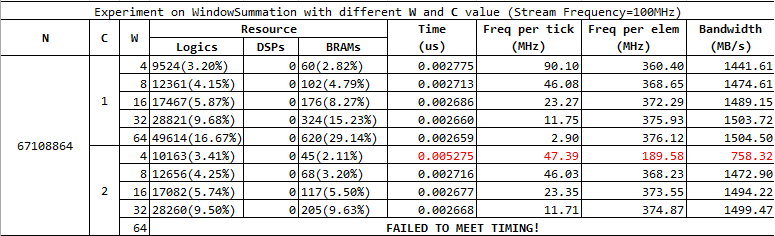
\includegraphics[width=1.0\textwidth]{window-summation}
\end{figure}

\section{Conclusion}
Multi-pumping as a resource sharing technique, could be supported in HLS system originally, and also it has been discovered that in code-level we could also use multi-pumping to save space harmlessly. The methodology about implementing multi-pumping on MaxJ could serve as code template and it's possible to use this template to multi-pump any kinds of "faster" components. It has been proved that kernel with multiple DSPs and ROM read ports could be multi-pumped seamlessly.

In the next chapter, I will mention this multi-pumping practice on SpMV, a much complexer problem then these 2 examples, about how could we find the resource bottleneck and how to reduce them by using multi-pumping. In the last chapter, this multi-pumping technique will be described and implemented in 2 simple serialization primitives, in Ruby HDL programming language. And the most important part is we could generate practical multi-pumped MaxJ code from this \textit{theoretical} HDL language.

\chapter{SpMV}
The focus of this SpMV project is not to provide the fastest SpMV implementation for some specific purpose, like what most other SpMV papers do. Here this project will have a general purpose implementation, which could handle most sparse matrix cases, with pretty good performance(May not be fastest though). The format of sparse matrix that I choose to use is called Blocked Compress Sparse Row(BCSR), which generates blocks upon CSR format. This chapter I'll first describe what is BCSR format and my MaxJ implementation of this format, experimental data will also be shown here. At last, we'll integrate our multi-pumping techniques with this SpMV implementation to see whether we could get better resource usage.

\section{BCSR Format}
This format could be generalized as a blocked version of CSR format. To generate a CSR representation of a sparse matrix, we could simply align the non zero elements to the left(or the other side if you wish). Here's an example sparse matrix, where those letters are representing non zero matrix elements.
\[
A = 
\begin{bmatrix}
	a & 0 & b & c \\
	d & e & f & 0 \\
	0 & 0 & 0 & g \\
	0 & h & i & 0
\end{bmatrix}
\]
And if we want to build a CSR represenation of this matrix, we could just pull all the non zero elements to the left. 
$$A_{csr} = 
\begin{bmatrix}
	a & b & c \\
	d & e & f \\
	g \\
	h & i
\end{bmatrix}
$$
It depends on yourself about how to store the CSR format, basically, it's just a 2 dimensional array, with each element as a pair of value and original column index. For the previous CSR example, the storage format could be: 
$$
\begin{bmatrix}
	(a,0) & (b,2) & (c,3) \\
	(d,0) & (e,1) & (f,2) \\
	(g,3) \\
	(h,1) & (i,2) \\
\end{bmatrix}
$$

These format works for many different matrices, and platforms, but its main deflect is that it will not be padded, and this is obviously not good for parallel processing units, especially our DFE design. So we choose to use BCSR format, which will pad zeros to each row, to align and group non zeros and padding zeros to blocks. The BCSR format with 2X2 block of the previous matrix is:

$$
\begin{bmatrix}
	(a,0) & (b,2) & (c,3) & (0,0)\\
	(d,0) & (e,1) & (f,2) & (0,0)\\
	(g,3) & (0,0) \\
	(h,1) & (i,2) \\
\end{bmatrix}
$$

With this format, we could simply pass one block to DFE in one tick. The further question is, how could we process $R\times C$ shape block in one tick?

\section{BCSR on FPGA}

The first thing we must specify is about where to put the data. Although Maxeler board has a lot of BRAMs to use, it will still be insufficient if we simply put all the storage on board. The simplest approach is to put vector value on BRAMs, and set input streams to take BCSR's index and value streams. So for each tick, each input stream will take $R\times C$ number of elements if the block has been configured as $R\times C$ shape.

\begin{figure}[h!]
  \caption{BCSR one block computation}
  \centering
    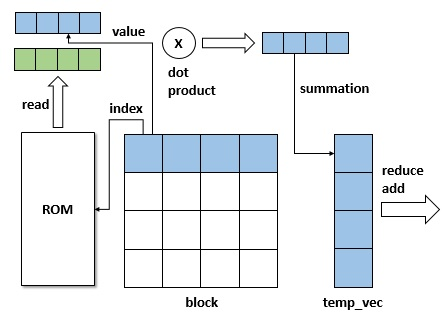
\includegraphics[width=0.5\textwidth]{bcsr}
\end{figure}

\subsection{3 steps calculation}
For each tick, the BCSR implementation will mainly do 3 things:
\begin{enumerate}
\item \textbf{Read from ROM}: For each row in the block, we use original column index to read value from vector, which has been stored on ROM.
\item \textbf{Multiply}: After read a size $C$ vector from ROM, we do multiplication between this little vector and the value from the row we're calculating. You could view this as the first step of dot product.
\item \textbf{Summation}: Then we do the second step of dot product, sum up the result vector we get from the previous step.
\end{enumerate}

If we have multiple rows to calculate in one tick, then we apply these 3 steps in parallel. And here's a wireframe of 4 X 4 block configuration.

Of course, we could describe this design in MaxJ kernel code(Listing 2.1). In this code snippet, the function \lstinline{summationTree} will generate a tree-like summation circuit, which has $log_2(C)-1$ level of adders, and in level $i = 0...log_2(C)-1$ will contains $2^i$ adders.

\begin{lstlisting}[caption=BCSR kernel]
for (int i = 0; i < R; i ++) {
	// gather	
	for (int j = 0; j < C; j++)	
		vectorValue[j] <== ROM.read(index[i*R+j]);
	// multiply
	for (int j = 0; j < C; j++)
		productValue[j] <== vectorValue[i] * rowValue[j];
	// summation
	result[i] <== summationTree(productValue, 0, C-1);
}
\end{lstlisting}

And each line could have multiple blocks, we need to sum up the \lstinline{temp_vec} to get the final result for each row, which is initially a reduce add operation. 

\subsection{Problems}

This BCSR design looks good, but it has several deflects: First, it can't handle large sparse matrix computation. As large matrix has large column size, which means we need to store a large amount of vector data inside ROM. And also, as we need to do multiple read in one tick for each block($R\times C$ times), we need to have $\frac{R\times C}{2}$ number of ROM copies as each ROM could only support 2 read ports in one tick. That's a huge amount of data and there's no sufficient place for these BRAMs. And also, as we're streaming matrix data in, the maximal bandwidth of PCIe will restrict our performance as our design could always process data elements faster.

\begin{figure}[h!]
  \caption{BCSR new architecture}
  \centering
    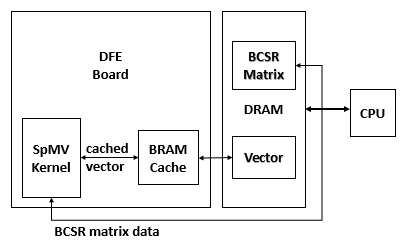
\includegraphics[width=0.7\textwidth]{bcsr-opt}
\end{figure}

So the main problem is about storage and bandwidth, and the major solution to this problem is by using LMem, a outside DRAM for DFE, which has large storage and connect with DFE with 20x more bandwidth. As LMem do not support random access, which is quite essential for ROM read of SpMV, we use an on-board BRAM cache to handle random access(Although this need more reordering on matrix). Here's the optimized architecture of our BCSR design(Figure 2.2).

\subsection{Multi-Pumping optimization}
If you take a closer look at our 3 steps BCSR calculation, you could find out that there're 2 steps that match our multi-pumping examples: one is \textbf{gather}, where we could multi-pump the ROM read, and \textbf{multiply}, those DSPs could be multi-pumped. Our BCSR SpMV will benefits a lot from this: It uses many ROM to do multiple reading and many DSPs to do dot production, with multi-pumping we could highly reduce those resource usage. And also, the \textbf{summation} operation is quite slow if we apply block configuration with large C value, which means our multi-pumped components could run at more than 2x clock rate of that slow clock rate. 

This part of work is still under evaluation, and may not be released until everything works fine.

\section{Experimental Study}

Experiments on this SpMV application are focusing on two aspects: One is about the maximal speed we could get, and some discovery about different parameters' could affect the performance. The other one is on the resource usage of our multi-pumping application, mainly on DSPs usage, we try to find out whether the resource usage will be reduced by using our multi-pumping design.

\subsection{Basic performance experiments}
According to our algorithm and design, if there's no bandwidth limitation(or comparing to our speed, its much faster), then the performance should be estimated as:
$$ \text{Estimated Frequency} = \text{Frequency} \times R \times C $$

So if we use $R$ and $C$ with the same $R \times C$ value, then the performance shouldn't be different. We evaluate the performance with 3 different metrics, suppose the runtime for each non-zero element is $T$:
\begin{enumerate}
\item \textbf{Bandwidth}: Bandwidth is the number of bytes that has been transferred in one second. In our application, on BCSR non zero pair will take 6 bytes, as 4 bytes for float value and 2 bytes for \texttt{uint16\_t} type index.
$$\text{Bandwidth} = \frac{6}{T}\times 10^{-6} (\text{MB/s})$$
\item \textbf{GFlops}: The effective floating point operation number will be two for each non zero element, one is for adder, the other is for multiplier.
$$\text{GFlops} = \frac{2}{T} \times 10^{-9} $$
\item \textbf{Frequency}: This is the real frequency we get from runtime. It should be close to our estimated frequency, although there will be some interferer while calculating.
$$\text{Frequency} = \frac{1}{T} \times 10^{-6} (\text{MHz})$$
\end{enumerate}

Here're the results we've got. We have tested 3 sets of $R\times C$ configurations: 16, 48 and 96. The reason we choose last 2 number is for the transfer between LMem and DFE(or CPU) should be divided by 384 bytes. And as C must be a number as power of 2, as the summation tree is a full binary tree, we need to fullfill every level. These data are based on several self-generated sparse matrices with number of columns as 8192 and total datasize equals to $8192^2$. We have generated dense matrices, triangle matrices, band matrices and random matrices. The performance result following are average results.

\begin{figure}[h!]
  \caption{BCSR LMem Performance}
  \centering
    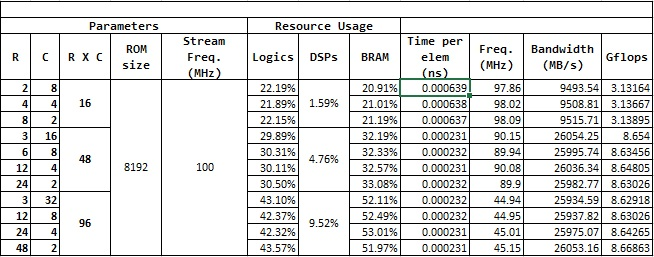
\includegraphics[width=1.0\textwidth]{bcsr-lmem-perf}
\end{figure}

For the performance, we could reach a maximal GFlops around 8.6, and there's a sharp frequency drop when we tried to use $R\times C=96$, which might meet the boundary bandwidth of LMem to DFE. The resource usage looks quite reasonable: The DSP usage is highly related to the $R\times C$ value, and so does the BRAM usage.

\subsection{Multi-Pumped BCSR SpMV}

Currently we have only tested the $R=4$ and $C=4$ with double pumped configuration. The one without multi-pumping will use 32 multipliers for calculation while the multi-pumped will only use half of them. 

\subsection{Others}

Other experimental data are stored in a spreadsheet, which contains the studies of ROM optimization, LMem optimization and bandwidth optimization of our SpMV BCSR algorithm. And also it includes those data which related to the previous CSRP format, the one that has been abandoned.

\section{Conclusion}
Our BCSR SpMV implementation could handle most of the sparse matrix cases, it do not depends on the distribution of number of non zeros in each row, and with the help of LMem and multi-pumping, we could store very large vector for calculation. Multi-pumping here not only reduces the DSP usage, but also reduce a large amount of BRAM usage, which is the resource bottleneck of our SpMV design. 

The way we apply multi-pumping on a non multi-pumped SpMV design suggests that our multi-pumping methodology will work perfectly, and could adapt to many different circumstances.

\chapter{Ruby}

Ruby is a highly abstract HDL language, which could write a very complex design in quite a few lines. Comparing to MaxJ, ruby code is much simpler and could help programmer concentrate on the design itself, without distracting on allocating memory, configuring and connecting input and output streams. But ruby don't have a powerful toolchain like MaxJ, which could use single command to deploy your hardware design on Maxeler FPGA board. So it's a good idea to combine these 2 languages together, with Ruby's simple syntax and MaxJ's toolchain. We could achieve this simply by translating Ruby code into MaxJ code, and do the compilation.

But as Ruby is highly abstract, there's no explicit configurations in the source code file, and Ruby itself doesn't contain optimization of the design, like what MaxJ do underneath. There'll be a conflict when MaxJ do pipelining implicitly, and Ruby wants to do cyclic loop on the pipelined operator. This problem will be covered later, and the solution will also be listed.

Ruby provides serialization methods, which could convert clock rate between the input and output ports of wires. If we simply translate one Ruby file into one MaxJ kernel file, then there'll be problem, as we have mentioned: MaxJ do not support multiple clock configuration on one kernel. And Ruby doesn't have kernel splitting primitives, we need to do this automatically. There's an algorithm that has been implemented to do this when translating Ruby code to MaxJ, the main idea is to split by clock rate changing, especially by \texttt{pdsr} and \texttt{sdpr} primitives. 

We could also use these 2 primitives to implement multi-pumping in Ruby. There'll be an example about how to do this in Ruby, and an example of translated MaxJ kernels and manager files could prove that our kernel splitting algorithm works.

\section{Cyclic loop problem}

\subsection{Background}
For those DSP components in MaxJ, they will be automaticlly pipelined by MaxCompiler. And if we do some cyclic loop with just one offset, then this circuit is faulty as we try to get a result which is currently in the pipeline.

And if we generate the MaxJ code for \lstinline{current = loop (add; DI 0; fork).}, then we will have a cyclic loop with 1 offset. There'll be problem if this \texttt{add} has been pipelined. The 1 offset before result we get are still in the pipeline when we get it.

Could we solve this problem without affecting the pipelining optimization? The answer is no. It's quite hard to generate a C-Slowed MaxJ code directly from Ruby, and without C-Slowing, the generated code will be really slow, as we are running the code with $\frac{1}{pipeline\ depth}$.

We could solve cyclic loop bug by using many solutions, but our approach is by setting the pipelining factor of this DSP to 0. We'll not have pipeline on this DSP then.

\subsection{Solution}

How could we know where exists the cyclic loop, and where to put our \texttt{push} and \texttt{pop} instructions? 

For the first problem, we could detect cyclic loop by using the input and output node number of each ruby gate, generated by ruby compiler. If the output node number is less than one of the input nodes number, then there definitely exists a cyclic loop. This feature is geranteed by Ruby compiler.

Here's the code snippet related to this solution:

\begin{lstlisting}[caption=Revision to fix cyclic loop]
(pushPipelineIfCyclic (inNodes, outp)) ^
(showGate (maxBackPatchForwardDeclaration) (device, input, output)) ^
(popPipelineIfCyclic (inNodes, outp))
\end{lstlisting}

The \texttt{showGate} function is the one output the string of MaxJ's assignment instructions, and we wrap this up if there's a cyclic loop within. Those \texttt{pushPipelineIfCyclic} or pop functions first detect the input nodes of this current gate, if this gate contains input nodes \texttt{inNodes} that is larger than the output nodes \texttt{outp}, we will output a string that push/pop pipelining factor 0.

\begin{lstlisting}[caption=Implementation of cyclic loop detector]
fun isCyclicLoop(inNodes, outp) = 
    List.foldl (fn (x, b) => ((x > outp) orelse b)) true inNodes

fun pushPipelineIfCyclic (inNodes, outp) = 
    if isCyclicLoop(inNodes, outp) 
    then "   optimization.pushPipeliningFactor(0);\n" 
    else ""

fun popPipelineIfCyclic (inNodes, outp) = 
    if isCyclicLoop(inNodes, outp) 
    then "   optimization.popPipeliningFactor();\n" 
    else ""
\end{lstlisting}

\subsection{Restriction}

As I've mentioned before, this solution is far from perfect. We simply banned pipelining, and the direct result would be a tremendously low maximal frequency we could achieve, especially we want to do complex design.

\section{Serialization primitives translation}

Most of the ruby's serialization primitives work fine while we're translating them from ruby to MaxJ, for example, \texttt{DI} the delay unit will be translated to \texttt{stream.offset} as what we expect. However, there're 2 more primitives that can't be correctly translated: \texttt{pdsr} and \texttt{sdpr}.

\subsection{Background}

\texttt{pdsr n} is a primitive which takes a n list of elements, and output 1 by 1 in the following n cycles. And \texttt{sdpr n} do things in reverse, they take n elements and output a n list in one cycle. The reason why this is not supported is that, the current ruby to MaxJ translation code could only support one kernel generation, \texttt{pdsr} and \texttt{sdpr} need to change the clock rate between those input and output ports. As we know that we could only assign one clock rate for one kernel in MaxJ, so it's impossible to do this if there's no multiple kernels generation mechanism supported.

Things are more difficult as there's no primitives that support kernel partition functionality. Programmers couldn't assign which part of the ruby circuit should be in one kernel. So we should choose whether to revise the ruby syntax and compiler itself, or detect kernels by some heuristic methods. We choose the second one.

\subsection{Graph labeling algorithm}

Currently, the main purpose of our kernel partitioning is due to clock rate changing while we're translating serialization ruby primitives to MaxJ. It's obvious that we should first(and maybe the last) to detect kernel border by using clock rate. So first of all, we need to generate a graph, or more precisely, a DAG that contains clock rate information. 

We build a graph from the raw output from ruby compiler first, which is called \texttt{pcircuit}. It contains the basic information of one ruby file. This data structure contains 3 components: 2 expressions of domains and ranges, and the relations in ruby code. We should know that there're 2 levels of circuit organization in ruby: The first level is called gate, which contains input and output ports, and one single processing unit(sort of). And the second level is called relation, which contains many gates, and all these gates are connected in parallel, which means they will not have dependencies to each other. The expression is another special type \texttt{expr}, it contains many constructors, but we mainly use the \texttt{WIRE} to get the wire id.

Start from input nodes, we could "flow" from input to output of the ruby file, and during this flowing procedure, we could met \texttt{pdsr} or \texttt{sdpr}, and they will change clock rate from input to output. So if we build have a initialized clock for input wires, and change or remain the same clock rate as the previous wire, then we could build a global graph labeled with clock rate.

\begin{lstlisting}[caption=Build labeled graph]
val (eL1,iL1) = appendEdgesToEdgeList (exprToEdges dom) []
val (eL2,iL2) = appendEdgesToEdgeList (exprToEdges ran) eL1
val g         = appendRelsToGraph rels ([], eL2)
val setClk    = initGraphClock 1.0 g
\end{lstlisting}

This code snippet lies in the main procedure of our kernel partitioning algorithm, as the initilization steps. It first append input and output nodes to the graph, and then append relation to build the edges between nodes. At last it will initialize the clock rate for each edge.

\subsection{Kernel partitioning algorithm}

Then we could partition our built graph. As we intends to split the graph by using different clock rate as boundary, the we could start from the input nodes, and mark all those edges which contains different clock rate in input edges and output edges as \textbf{boundary}. The tricky point of this algorithm is, it will stop immediately when we met one different clock rate node, just like a wavefront.

Here's a diagram to show this(Figure 3.1). The components in the dashed rectangle should be partitioned as a new kernel. And all the components outside the 2x clock rate box should be integrated in one. 

\begin{figure}[h!]
  \caption{Diagram of kernel partitioning}
  \centering
    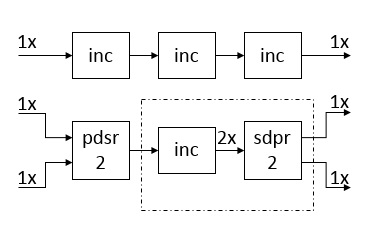
\includegraphics[width=0.5\textwidth]{pdsr}
\end{figure}

This is the code snippet to do this. It's prefixed with iter as this function will iteratively build the graph. It takes a list of input nodes, and start with input nodes to take all those edges and nodes it met as a graph. It will stop in 2 circumstances: output or met clock rate border. The history list will store those input nodes it has met to avoid infinite loop.

\begin{lstlisting}[caption=Iter partitioning algorithm]
fun iterSplitGraph [] hs g = []
    | iterSplitGraph es hs g =
    ( let 
        val splitEdgeIds = iterFindSplitEdges es g
        val splitNewGraph= splitAndFilterEdgesInGraph splitEdgeIds g
        val newInEdgeIds = getGraphInputEdges splitNewGraph
        val nextHistory  = es @ hs
        val nextInEdgeIds= 
			filterExistEdgeList 
				(getListCompliment nextHistory newInEdgeIds) 
				splitNewGraph
        val build        = iterBuildGraph es splitNewGraph ([],[])
        val retGraphList = iterSplitGraph nextInEdgeIds nextHistory splitNewGraph
      in 
        build::retGraphList
      end )
\end{lstlisting}

\subsection{Result: Multi-Pumping in Ruby}

Besides this, we also need some functions to support manager and cpu code printing. I'll not mention them here, but it should be mentioned that the printer function works fine and we could run MaxJ simulation directly from ruby file(by using some Makefile configuration of course).

\begin{figure}[h!]
  \caption{Diagram of ruby multi-pumping example}
  \centering
    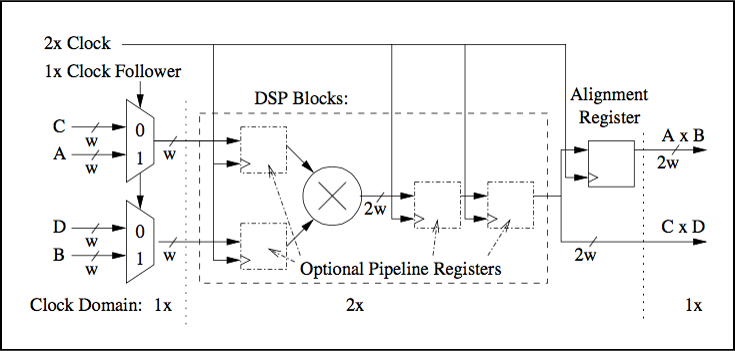
\includegraphics[width=0.6\textwidth]{toronto}
\end{figure}

Here's an generated example of ruby multi-pumping and the generated MaxJ code. Here we will multi-pump one multiplier, make it serve 4 input streams, just like this example(Figure 3.2). If we ignore those pipeline registers and multiplexers, we could build this circuit by using this ruby code:

\begin{lstlisting}
current = [pdsr 2, pdsr 2]; mult; sdpr 2.
\end{lstlisting}

Here're the generated MaxJ code. There'll be 2 kernel files generated, the first one only handles the input stream and by using pdsr, we could merge these 4 streams in 2 streams. Then the second kernel will run at 2x clock rate to take the input streams, and do multiplication. 

\begin{lstlisting}[caption=Generated MaxJ code]
public class CurrentManager extends CustomManager {

public CurrentManager (EngineParameters params) {
   super(params);

   // kernel block declarations:
   KernelBlock k0 = addKernel(new Kernel1(makeKernelParameters("Kernel1")));
   KernelBlock k1 = addKernel(new Kernel2(makeKernelParameters("Kernel2")));

   // kernel block clocks declarations:
   float clk = 100;
   config.setDefaultStreamClockFrequency((int)clk);
   ManagerClock clk0 = generateStreamClock("clk0", (int)(clk * 1.0));
   k0.setClock(clk0);
   ManagerClock clk1 = generateStreamClock("clk1", (int)(clk * 2.0));
   k1.setClock(clk1);

   // DFELinks declarations:
   addStreamToCPU("board2cpu_0") <== k1.getOutput("out4");
   addStreamToCPU("board2cpu_1") <== k1.getOutput("out3");
   k1.getInput("inp6") <== k0.getOutput("out2");
   k1.getInput("inp5") <== k0.getOutput("out1");
   k0.getInput("inp4") <== addStreamFromCPU("cpu2board_0");
   k0.getInput("inp3") <== addStreamFromCPU("cpu2board_1");
   k0.getInput("inp2") <== addStreamFromCPU("cpu2board_2");
   k0.getInput("inp1") <== addStreamFromCPU("cpu2board_3");

   createSLiCinterface(interfaceDefault());
} // end constructor
\end{lstlisting}

\begin{appendices}
\chapter{Weekly Report Archive}

\subsection{Report of Week 3 (Aug. 3, 2015)}

Basically I've finished running and testing the real hardware implementation of my previous SpMV design, and improved it by enabling large matrix calculation. Also, I've written a simple multi-pumped design by using MaxJ. This one has been checked about its accuracy and time frequency. 

\subsubsection{SpMV Implementation}

\paragraph{CSRP format} The format that I've devised and implemented could be called as CSRP (\textit{CSR format with Padding zeros}). This format enables multiple rows of elements to be calculated at the same time, and when those simultaneous caculated rows don't have the same number of non-zeros, this format will automatically add padding zeros to ensure the result is correct. 

The main advantage of this format is its simplicity in implementation, but it will also face these deflects:
\begin{enumerate}
\item \textit{Redundant calculation}: For those cases when different rows have quite different number of non-zeros, the total number of calculations will depend on the maximum number of non-zeros among these rows. 
\item \textit{Resource duplication}: We need to replicate same kind of resources to enable parallelized calculation. 
\end{enumerate}

\paragraph{Implementation} The implementation of CSRP format is quite simple. We set 2 input streams, one is for value and the other is for column index of each non-zero element. All these input streams are interleaved and zero-padded. Each of the calculation components has one a cyclic-loop which will sum the result for current row, and one ROM which stores the values of vector. We take Matrix Market Format of matrix as input, and generate interleaved data from the original data. 

\paragraph{Optimization} The detailed statistics will be updated by next week, but here I'll list several ideas of optimization:
\begin{enumerate}
\item \textit{Reduce redundant calculation}: Currently the number of redundant calculation depends on the maximal number of non-zeros of all rows in the matrix. We could reorganize our output data and let number of padding zeros depend on the maximal number of non-zeros of all rows in each simultaneously calculated groups. After that, we could also reorder the matrix rows to get the best placement of rows into different groups, and get a globally optimizated result.
\item \textit{Reduce resource usage}: We could do this by using dual-port of ROM, and if possible, using multi-pumping.
\end{enumerate}

\paragraph{TODO} 
\begin{enumerate}
\item Finish the fully implemented baseline by Thursday. Fully implemented means, it could take MMF matrix data as input, and has reasonable space of memory.
\item Finish the first kind of optimization and the dual-port version by the end of this week.
\item If possible, try a multi-pumped version. (Only after the first 2 tasks finished)
\end{enumerate}

\subsubsection{Multi-Pumping}

\paragraph{Simple implementation} This simple implementation will do square on 2 input streams. Those input streams will be configured at 1x clock rate, and the inner multiplier will be configured at 2x clock rate. It could be implemented by using \texttt{ManagerClock} in MaxJ. The real hardware implementation has also been checked. The result is correct but the frequency is not accurate.

\paragraph{TODO}
\begin{enumerate}
\item Finish checking this simple implementation. Must get a reasonable clock frequence.
\item Finish a Ruby implementation of multi-pumping by Thursday. Also, generate its MaxJ code.
\end{enumerate}

\subsubsection{Ruby Compiler}

I haven't checked the compiler last week, but I'll start it as soon as possible. Basically, I should first use ruby to do some basic design, compile it into MaxJ and run it. After that, try to do some loop in Ruby. And test its MaxJ result (Which may not be correct).


 	\newpage

\subsection{Report of Week 4 (Aug 4th, 2015)}

This week I've made progress on all the 3 directions: SpMV in MaxJ, multi-pumping in MaxJ and multi-pumping in Ruby. Here're the details.

\subsubsection{SpMV in MaxJ}
According to the plan, I've finished the baseline version of CSRp SpMV on time. You could find out the definition of CSRp in the archived week 3 report. This version will generate correct result, but it must be improved in many aspects:
\begin{enumerate}
\item 
\textbf{Get runtime correct}: Currently, if we add level of parallelization, the run time will increase, not as what we expected. If the code is correct(maybe not), then something wrong might happen during synthesis and implementation. Check the \textbf{clock frequency} of the \textbf{built kernel}. This will tell whether there's problem during the implementation: if the clock frequency also not follow our expectation.

It might be the case that the current using matrix will never benefit from the level of parallelization, so we need to generate matrix based on our current design specification, and discover their performance.

\textbf{Todo} First check out the frequency of each design with different parallelization level. Also try to organize the code better.Then use randomized benchmark, not only the value, but also the structure to test run time result. 

\item
\textbf{Improved CSRp format}: The CSRp format will perform really bad if the padded zeros occupy most of the computations, which means, we have lots of redundant zeros. Why we have those zeros? As we cannot calculate all the rows simultaneously, only part of the rows will be calculate at the same time. If we call these rows a \textbf{block}, then we will calculate the whole matrix block by block. Now, we do not specifically add \textbf{splitters} between those blocks. We would know which block we are calculating only by forcing all the blocks has equal width. The way we force this happen is by padding zeros. The number of padding zeros could be enormous if we have a very wide block and most of the blocks are quite narrow. The \textbf{redundancy} metrics could be calculated by using:

\[ R_{CSRp}(N) = 
	\max_{0 \leq i < N}(block_i.width)\times N \times p - 
	\sum_{i}^{Np} row_i.width 
\]

where N is the number of blocks, and p is the level of parallelization. If we have N and p assigned, then the whole number of rows should be Np. The \textbf{width} is the number of non-zeros for each row or block. Especially for blocks, their width is the maximal width among all rows in that block.

Obviously, we could improve this. If we assign more information for each clock cycle, like "whether this cycle is in the end of one block", which is the \textbf{splitter} that we have mentioned above, then we do not need to do padding on all the blocks to make sure they have same width.

This one could be achieved by adding a new input stream of 0, 1 boolean values. We could verify the improvement in speed and space increasement.

\textbf{Todo}: Finish the first part of SpMV work first. And build this design later. Discover their performance differences. And I think this is one should be the standard design of \textbf{baseline}. Previous one has really bad performance.

\item
\textbf{With multi-pumping}: I've already finished a multi-pumping MaxJ version, which has a simple multiplier inside. And we all know that SpMV is all about add and multiply(basically), so we could use the same framework to optimize this SpMV design.

\textbf{Todo}: Last one to do, I think I could do this in the next week.
\end{enumerate}

That's all about this week's SpMV work, I'll attach a full chart about this design's performance in next week's report, as I need to verify some current data this week.

\subsubsection{Multi-pumping in MaxJ}
 	\newpage

\section{Report of Week 5 and 6}
\subsection{MaxJ SpMV Implementation}

Compressed Sparse Row(CSR) is a famous sparse matrix storage method, it pull all the non zeros to the left of their own row, and store their original column index before they have been aligned. I'm building my SpMV algorithm based on this format. 

\subsubsection{CSRP format introduction}
In order to reduce complex control logic which could slow down the processing and introduce bugs, there'll be \textbf{padding} zeros at the end of each row, in order to make those rows, which will be processed together, have the same number of elements to calculate(although there'll be some useless zeros). That's the idea about CSRP format.

\subsubsection{Redundancy formalization}

If we align all our rows to the row with maximal number of nonzeros, then we could imagine there'll be lots of redundancy. As we will process only a small number of rows at the same time(number of pipes), we could just align rows to the longest row in each \textbf{processing group}.

Let's formalize this description: If we have N rows for one sparse matrix, and for row $i$ it has $L_i$ number of non zeros. And if we group all these rows by $R$, which is the number of pipes for our design, then all these $R$ rows in one group will be calculated together. So we could devise this formula:

The lower bound of our \textbf{redundant} calculation cycles will be:
\begin{equation}
Redundant\ cycles = \sum_{i}^{N/R} R \times \max_{j}^{R} L_{i\times R + j} - \sum_{i}^{N} L_i
\end{equation}

\subsubsection{Redundancy Optimization}

If we transform formula (1) to this form:

\begin{equation}
Redundant\ cycles = \sum_{i}^{N/R} (R \times \max_{j}^{R} L_{i\times R + j} - \sum_{j}^{R} L_{i \times R + j})
\end{equation}

So here's a heuristic rule: we need to make sure there's no such case, that a very long row and several short rows coexist in one group. According to this idea, we could simply do a \textbf{sorting} on the rows by their length(which is a greedy algorithm). Is this really the best solution? We could easily prove it. 

Imagine that we have $N/R$ "buckets", each bucket could contain $R$ rows. And now we need to put rows inside those buckets. We suppose that the best solution is put rows one by one in the sorted sequence, which means that the rows in the first group will be the rows with top $R$ number of non zeros.

If there's a better solution than this one, then it should have swapped some of its elements. If we swap 2 rows between 2 groups, then it will increase redundancy in both groups.

\subsubsection{Performance}

I've tested this format with different $R$ value, and 2 extreme sparse matrix format: dense and triagle. The following features have been discovered:
\begin{enumerate}
\item The maximal performance I could get is by using design with $R$ equals to 32, and for dense matrix, GFlops is 0.28, for triangle matrix, it's 0.22.
\item With larger $R$ value, the performance increase at first, and the fall down.
\item If $R$ is larger, then redundancy will be larger.
\end{enumerate}

More detailed test and report will be attached once I've finished the final version.

\subsection{Ruby Multi-Pumping Implementation}

In this section I'm going to make a summary about current progress on Ruby multi-pumping. 

\subsubsection{Ruby serialization primitives}

If we want to implement multi-pumping in Ruby, the first thing we must specify is: how could we have different clock rate in Ruby? The basic primitive about clock rate changing is \texttt{pdsr} and \texttt{sdpr}. The first one will change a n length list to n cycles of one element output, which will slow down the clock rate to 1/n. The \texttt{sdpr} will perform reversely.

\subsubsection{Perspectives}

Just take one simple example. If we want to multi pump +1 operation, and as inc(which is +1) has only 1 input and 1 output, then we could simply decide that the input for multi pumped inc is <x, y>, a 2-list. 

Here're 2 different approach:
\begin{enumerate}
\item \textbf{Single kernel}: we just have one kernel which runs at 2x clock rate, and 2 input streams has interleaved, 1x clock rate input.
\item \textbf{Multi kernel}: we run the kernel at 2x clock rate, but the input stream will run at 1x clock rate.
\end{enumerate}

Here's an example, for the single kernel approach, the input would be like: $\mathtt{<x_0,\_>, <\_,y_0>,<x_1,\_>,<\_,y_1>,...}$. Please notice that this stream runs at 2x clock rate. For the second approach, we will have $\mathtt{<x_0,y_0>,<x_1,y_1>,...}$ as input stream, and this stream will run at 1x clock rate.

The first one is simple but not so general. The second one is more accurate and harder to implement, especially for Ruby to MaxJ translation, as we need to generate manager and kernel at the same time.

\subsubsection{Implementation}

Here I'll introduce the solution for the second approach, which will be the test case of our Ruby to MaxJ translation function.

First we need to change the clock rate of input, which could be implemented by using \texttt{pdsr 2}. And then, do inc for each element. At last, use \texttt{sdpr 2} to bundle 2 output as 1.

Here's a single line of code: \lstinline{current = pdsr 2; inc; sdpr 2.}

\subsection{Ruby cyclic loop}

This part is about fixing the bug of cyclic loop in Ruby.

\subsubsection{Problem: MaxCompiler auto-pipelining}

For those DSP components in MaxJ, they will be automaticlly pipelined by MaxCompiler. And if we do some cyclic loop with just one offset, then this circuit is faulty as we try to get a result which is currently in the pipeline.

And if we generate the MaxJ code for \lstinline{current = loop (add; DI 0; fork).}, then we will have a cyclic loop with 1 offset.

We could solve cyclic loop bug by using many solutions, but our approach is by setting the pipelining factor of this DSP to 0. We'll not have pipeline on this DSP then.

\subsubsection{Solution}

How could we know where exists the cyclic loop, and where to put our \texttt{push} and \texttt{pop} instructions? 

For the first problem, we could detect cyclic loop by using the input and output node number of each ruby gate, generated by ruby compiler. If the output node number is less than one of the input nodes number, then there definitely exists a cyclic loop. This feature is geranteed by Ruby compiler.

For the next problem, just insert push and pop before and after the calculation part. 	\newpage

\section{Report of Week 7}

\subsection{What is BCSR?}
BCSR is a sparse matrix format which is based on well-known CSR format. It's basic element is little block of non-zeros, just like cutting CSR to little blocks. Each block has a shape of $r \times c$, where r and c's value will not be so large. 

The BCSR format contains 2 main procedures, one is converting, which will transform a traditional COO format to BCSR format storage. The other one is computing, which will do computation on BCSR format.

\subsubsection{Convert}
The convert procedure will act like this, for example here's a sparse matrix A:
\[
A = 
\begin{bmatrix}
	a & 0 & b & c \\
	d & e & f & 0 \\
	0 & 0 & 0 & g \\
	0 & h & i & 0
\end{bmatrix}
\]

If it's a CSR format, the final result would be:
\[
A_{csr} = 
\begin{bmatrix}
	a & b & c \\
	d & e & f \\
	g \\
	h & i
\end{bmatrix}
\]

And for a BCSR format, the result would be:
\[
A_{bcsr} =
\begin{bmatrix}
	a & b\\
	d & e
\end{bmatrix}
,
\begin{bmatrix}
	c & 0\\
	f & 0
\end{bmatrix}
,
\begin{bmatrix}
	g & 0\\
	h & i
\end{bmatrix}
\]

\subsection{BCSR Performance}

Let's check out the maximal performance we could get if this design is IO-bound. If the PCIe bandwidth is 2GB/s, and we'll input 2 32-bits data, one for index, the other one for value, for each non zero. So we could process data per second:
$$ \text{Non zero per second} = \frac{2(GB/s)}{2\times4(Byte)} = 0.25(G/s) $$

And for each non zero, we will have 2 floating point operations(adder and multiplier), so the maximal GFlops we could get is:
$$ \text{GFlops} = 0.25 (G/s) \times 2(Flop) = 0.5 $$

\subsubsection{Multi-pumped BCSR design}

Referring to the BCSR format, we will calculate multiple multiplication in one single tick, which is a brillliant feature to be multi-pumped. But due to the constraints of MaxCompiler, we need to have multiple kernel blocks now, as we could only assign one universal clock rate to each kernel. We could divide this multi-pumped BCSR design into 3 parts:

\begin{description}
\item[Gather] For each pipe, we need to gather the input vector and value vector. Input vector means the values in the vector parameter, read from ROM. 
\item[Multiply] We send those input and value vectors to this multiply part, and this part runs at 2x clock rate, which is the computation core of multi-pumping design.
\item[Sum] Will take result from multi-pumping multipliers and use summation tree to sum them up. It will also take a \texttt{start} stream to denote whether the current calculated block is the start of each group.
\end{description}

\subsection{Ruby serial primitives}

This part of work is about how to compile Ruby serial primitives to MaxJ code, mainly \texttt{pdsr} and \texttt{sdpr}. 

\subsubsection{\texttt{showGate} and Function Device}
\texttt{showGate} is the core function to generate the MaxJ expression of a Ruby circuit. For instance, \texttt{add} primitive will be transformed to "+" by using \texttt{showGate}. But things will be different for \texttt{pdsr} and \texttt{sdpr}, as \texttt{showGate} currently could only support infix, eq and some other basic primitives, there's nothing like "function" has been supported, which will be quite useful to definie \texttt{pdsr} and \texttt{sdpr}.

Briefly, my approach is:
\begin{enumerate}
\item Add a condition filter \texttt{isFunc} in \texttt{showGate}, to check whether the current device is a \textbf{function device}, which should be implemented like \texttt{func(t1, t2)} in MaxJ. 
\item Append the builtin function definition backward in the kernel class definition. 
\end{enumerate}

\subsubsection{\texttt{pdsr} and \texttt{sdpr}}
How to define these 2 primitives in MaxJ? The simplest way is using a combination of \textbf{counter} and \textbf{mutiplexer}, which should be \texttt{simpleCounter} and \texttt{mux} in MaxJ. A simple definition for \texttt{pdsr 2} is:

\begin{lstlisting}
private DFEVar pdsr2(DFEVar t0,DFEVar t1) {
  DFEVar counter = control.count.simpleCounter(
    			MathUtils.bitsToAddress(2));
  return control.mux(counter, t0, t1);
}
\end{lstlisting}

This snippet of code is auto-generated, and suit for different value of n in \texttt{pdsr n} expression.

But for \texttt{sdpr}, things will be different, as no 2 or more number of output ports device will be supported in \texttt{printmax}, I think maybe it's better to optimize this by using \texttt{DFEVector}. 	\newpage

\end{appendices}

\bibliography{report-bib}
\bibliographystyle{acm}
\end{document}
